%%%%%%%%%%%%%%%%%%%%%%%%%%%%%%%%%%%%%%%%%
% University/School Laboratory Report
% LaTeX Template
% Version 3.1 (25/3/14)
%
% This template has been downloaded from:
% http://www.LaTeXTemplates.com
%
% Original author:
% Linux and Unix Users Group at Virginia Tech Wiki 
% (https://vtluug.org/wiki/Example_LaTeX_chem_lab_report)
%
% License:
% CC BY-NC-SA 3.0 (http://creativecommons.org/licenses/by-nc-sa/3.0/)
%
%%%%%%%%%%%%%%%%%%%%%%%%%%%%%%%%%%%%%%%%%

%----------------------------------------------------------------------------------------
%	PACKAGES AND DOCUMENT CONFIGURATIONS
%----------------------------------------------------------------------------------------

\documentclass{article}

\usepackage[version=3]{mhchem} % Package for chemical equation typesetting
\usepackage{siunitx} % Provides the \SI{}{} and \si{} command for typesetting SI units
\usepackage{graphicx} % Required for the inclusion of images
\usepackage{natbib} % Required to change bibliography style to APA
\usepackage{amsmath} % Required for some math elements 
\usepackage{todonotes}
\usepackage{wrapfig}
\usepackage{geometry}
\newgeometry{left=2cm, right=2cm, bottom=2cm}
\setlength\parindent{0pt} % Removes all indentation from paragraphs

\renewcommand{\labelenumi}{\alph{enumi}.} % Make numbering in the enumerate environment by letter rather than number (e.g. section 6)

%\usepackage{times} % Uncomment to use the Times New Roman font

%----------------------------------------------------------------------------------------
%	DOCUMENT INFORMATION
%----------------------------------------------------------------------------------------

\title{Energy Aware Software -- Research Plan} % Title

\author{Principal investigator: Simon Holmbacka\\ \AA{}bo Akademi University, Embedded Systems Laboratory} % Author name

\date{\today} % Date for the report

\begin{document}

\maketitle % Insert the title, author and date

\section{Rationale}
Energy efficiency in computer systems is currently a major concern in field computer engineering for several reasons such as increased frequency of the battery re-charge intervals, 
monetary cost because of high electrical consumption and thermal effects leading to increased cooling requirements with high noise levels. 
Furthermore, energy efficiency is also a concern for achieving increased performance. 
One of the performance limits in current microprocessors because the Dennard scaling [16 from thesis] is no longer valid. 
Dennard scaling forecasts that the power density of transistors stays constant as the manufacturing technology decreases. 
This means that as transistors become smaller, energy efficiency is improved by transistor technology such that the power remains in proportion to the area. 
In recent hardware, this scaling no longer applies since the voltage range used in transistors no longer can be lowered. 
The end of Dennard scaling brings consequences such as an unproportioned increase in thermal dissipation leading to dark silicon, 
which means that all processing power on a chip cannot be used simultaneously because of the limited power envelope.
To tackle these problems, power management systems are implemented to scale the performance of the system according to the current resource demand. 
Power management has traditionally been an area of research providing hardware solutions or runtime power management in the operating system in form of frequency governors. 
Energy awareness in the application software is currently non-existent. This means that applications are not involved in the power management decisions, 
nor does any interface between the applications and the runtime system to provide such facilities exist. 
Power management in the operating system is therefore performed purely based on indirect implications of software execution, usually referred to as the workload. 
Workload in operating systems is measured as a sliding window average over an active and idle CPU as illustrated in Figure~\ref{fig:workload}. 

\begin{figure}[h]
	\centering
	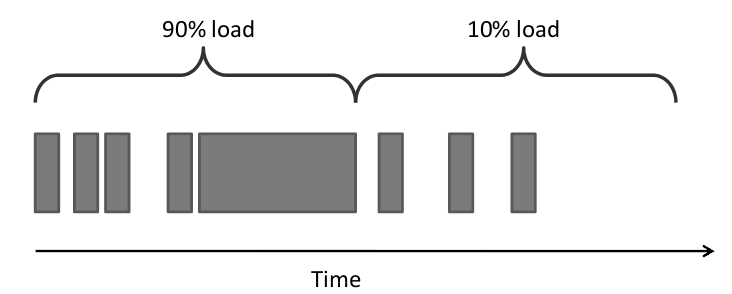
\includegraphics[scale=0.5]{fig/workload.png}
	\caption{Load calculated as a ratio between active and idle for a defined window (Gray rectangles represent an active CPU).}
	\label{fig:workload}
\end{figure}

The power management is then based on the idle percentage of such a window. 
Based on this, the hardware resources (for example in terms of increased clock frequency) are allocated as the percentage increases beyond a given threshold. 
The problem with this approach is that the workload does not describe resource requirements. 
For example, in case the CPU is set to decode a video, the workload will increase to 100\% as soon as the video frames are being decoded.  
This means that the CPU is clocked to the maximum frequency as long as the frames are being decoded and the decoded frame rate is only limited by the speed of the CPU; 
even if the required decoding rate is only 25 frames per second. In other words, the application will be executed unnecessarily fast. 
As results from \cite{HolmbackaHipeac, HolmbackaDasip} show, executing the application unnecessarily fast wastes significantly more energy than executing the application on a moderate, 
but still at a sufficiently fast, performance level. 
Executing applications on this performance level also decreases the thermal dissipation, and the overhead of performance level switches are significantly reduced.
The currently unsolved problem is to manage to execute an application on a moderate, yet sufficiently high, performance level. 
In order to execute applications at the most energy efficient performance level, additional knowledge about resource requirement must be set in the application. 
This is called making the application energy aware and is the proposed contribution in this research plan. To this date, no tool chain supports energy awareness in application software. 
This forces the runtime system to make blind decisions about power management only based on the system workload. 
Energy awareness, on the other hand, allows the application to express the required level of performance for functioning properly. 
For example, the video decoder requires a frame rate of 25 frames per second in order for the human eye to interpret the video as smoothly moving. 

\subsection{Application meta-data}
\todo[inline,color=orange]{Add this}

\subsection{Previous work}
I have worked the five past years on low power and energy aware software in the embedded systems lab in the \AA{}bo Akademi University. 
During these years I have put a special interest in mobile phone processors and their significance for energy awareness in general. 
This is because it has been noted that the trend of performance requirements by far exceeds the battery capacity of a mobile device, especially since the mobile multi-core revolution \cite{BatteryCapacity,CPUCapacity}. 
This means that the performance of the hardware and the demand for performance of the user is greater than the energy a battery with limited dimensions can physically store. 
Because of the slow capacity increase in batteries, the available energy must be used more efficiently in order for such a mobile device to retain its usability.
In my PhD thesis ``\textit{Energy Aware Software for Many-Core Systems}'' I presented two guidelines for creating energy aware software on modern many-core hardware. 
Implementing the recommendations in software has proven to reduce the energy consumption significantly without degrading the performance, especially on mobile multi-core hardware \cite{HolmbackaHipeac}. 
The recommendations called ``Energy aware mapping'' and ``Energy aware resource allocation'' are used to tailor the resource allocation to the software executing, 
and a prototype runtime system was implemented as a phase of the PhD thesis. 
Using this software, I implemented and released the Android app “Low Energy Player” on Google store\footnote{https://play.google.com/store/apps/details?id=org.videolan.vlc.LEL.lite.green} as a state-of-the-art demonstration of the work in my PhD work. 
This research is intended to go beyond the state-of-the-art by extending the prototype runtime environment to a proper framework for energy aware programming.

\subsection{Related work}
``Low energy programming'' or ``Low power programming'' has previously existed in the form focusing on the programming paradigm or on the programming syntax. 
Guidelines from Intel \cite{IntelLowPower} suggests the use of a certain level of loop unrolling, vectorization, memory intensity cache usage etc.
for achieving maximum energy efficiency in combination with intel compiler tools. 
Such recommendations are applied only on the algorithms in the program, and do not cover, the intention of the program for functioning efficiently together with the runtime system allocating the resources. 
The low power programming guidelines from Intel also require the programming to construct the program in a certain way in order to become energy efficient, 
and the underlying hardware architecture must be known. 
On the contrary, my framework for energy efficient programming requires minimal effort of the programmer and it is hardware agnostic. 
The only task of the programmer, using my framework, is to specify resource requirements using a simple library, whereafter the runtime environment allocates the required resources.

The \textbf{Carbon Research Group}\footnote{http://groups.csail.mit.edu/carbon/} at MIT has developed a heartbeat framework to evaluate performance as a generic parameter in software construction. The framework is capable of measuring performance of any application as a generic parameter by user inserted API calls to the heartbeat library. Measuring performance is the necessary first step when constructing a feedback-based control system. For example it enables the possibility to measure the framerate in a video decoder, but a controller is then needed to allocate the resources in order to keep the performance on a given setpoint. We consider using the heartbeat framework for measuring generic performance in our energy awareness framework, but we plan to extend the framework considerably in order to add the controller for allocating resources.\\

The \textbf{Hardkernel} project\footnote{http://www.hardkernel.com/main/main.php} creating the Odroid family boards recently released the Global Task Scheduling (GTS) support for the ARM big.LITTLE devices. “High performance threads” are scheduled to the big high performance cores and “Low performance threads” are scheduled to LITTLE energy efficient cores based on the workload activity of the threads in order to save energy. Even though the activity level of a thread is an early attempt introduce energy awareness in the system, the practical results are poor. In other words, the scheduler most often schedule a thread on “the wrong core”. This results not only in poor energy efficiency, but also in poor performance of the applications and poor user experience. We intend to use this platform as one of the reference models for our energy awareness framework because its SoC is very popular and is being used in millions of Android devices worldwide.\\

Our research group is currently a partner in the \textbf{INTERSYS} project\footnote{http://iot4health.utu.fi/?p=374} dedicated to standardize and optimize interconnected IoT devices handling streaming data. Since the number of IoT devices are expected to rapidly increase in the near future, the project is extending interoperability notions for handling the massive amount of data streams from small devices to gateways and servers. Still missing in the field of IoT is the notion of energy awareness, which is a crucial point as most devices operate on battery-only power and are expected to operate for long time intervals. We intend to work closely with this project and we plan to introduce the notion of energy awareness in IoT systems.\\

\textbf{EMBECOSM}\footnote{http://www.embecosm.com/} focus on providing the GCC compiler with the notion of energy efficiency, in practice this means learning which compiler flags that minimizes the energy consumption for a selected architecture. The outcome of this project is similar to OpenTuner [REF] from MIT, which is capable of offline optimization of multi-criteria problems. Both projects provide a metric for offline optimization, but runtime support, which we suggest, is not stated in their scope. Runtime optimization is critical in virtually any environment containing multi-node and heterogeneous multi-node platforms. This is because the data used in especially streaming applications like multi-media software is arbitrary or difficult to predict. Compile time optimizations can for example not predict what kind of video format is being used in a video decoder.\\

The \textbf{StarPU}\footnote{http://starpu.gforge.inria.fr/} project at INRIA Bordeaux has presented a runtime system to minimize the performance for heterogeneous architectures. The system builds a performance model of the implemented CUDA or OpenCL kernels based on benchmarking on CPUs and GPUs, after which the system is able to schedule the kernels onto the most performance efficient device. The \textbf{PEPPHER}\footnote{http://www.peppher.eu/} project has used StarPU as a backend and the outcome of the project is a tool capable of generating multi-variant tasks for StarPU (OpenMP, OpenCL etc.). However, StarPU only consider the optimizations in form of performance. When adding more complex criteria with multiple variables such as energy efficiency or cost, StarPU lacks the insight to such resource allocation.

\section{Objectives and expected results}
\subsection{Objectives}
My design recommendations for energy aware programming extends the application to signal resource requirements to the runtime system which allocates the hardware resources.
\todo[inline,color=orange]{Explain how it is used}
\todo[inline,color=orange]{Explain the meta data}
The objectives of my research is to create a framework for programming energy aware software. 
This means that a programmer is able to implement my low energy design recommendations by implementing a few lines of code in both newly designed and in legacy software.
The end-user of the software might- or might not be able to influence the decision process of the runtime system. 
Figure \ref{fig:netflix} illustrates for example the ability to add a Quality-of-Service option to the Netflix app running on Android. 

\begin{wrapfigure}{r}{0.4\textwidth}
  \begin{center}
    
\includegraphics[width=0.3\textwidth]{fig/netflix.png}
  \end{center}
  \caption{Quality-of-Service as a left click option in the Netflix app on Android}
  \label{fig:netflix}
  \vspace{-2cm}
\end{wrapfigure}
The user can use this option to select the trade-off between energy savings and performance in terms of decoding framerate or other parameters. 
Options can set based on a defined value like ``decoding framerate'' illustrated in Figure XXX \todo[color=green]{add these} or as a more abstract option as illustrated in Figure XXX \todo[color=green]{add these}. 
The intension of the energy aware framework is to expose the link between the application and the runtime system, while the design of using its abilities is up to the programmer.

\subsection{Hypothesis}
\todo[inline,color=orange]{Points here}

\subsubsection{Previous work on energy aware software}
In previous work, Eyerman et al. \cite{Eyerman:09} claim that no single throughput metric is fundamen tally generic for multiprogram workloads. 
Performance should instead be expressed as related to the internal single case-study; a direction adopted in this research. 
We plan to integrate this direction of thinking into user defined meta-data that expresses resource requirements in software.

In early research, a high-level language CQML \cite{Aagedal:01} was suggested for describing QoS requirements integrated in UML. 
CQML links a high level QoS description to system performance, and can describe system actions based on the result. 
Applications specify a performance setpoint and a lower bound acceptable performance level in context of the application. 
Applications then monitor own performance and signal this value to the QoS manager periodically. 
Similar notations as this the language will be considered in this research to describe QoS in applications, 
but more focus will put on the link between applications and hardware resources in a single computer system.
Our methods for energy aware programming will not be tied to a certain programming language and the framework itself will have the flexibility to be integrated from various programming environments such as servers and PC Linux and Android.

Hoffmann et. al propose heartbeats \cite{Hoffmann:10} as a generic performance parameter. 
The heartbeats are setup by including a set of heartbeat API calls in applications, which are used to monitor the application performance. 
By calling the heartbeat API on suitable places in the applications such as large loops, a notion of the update interval between API calls is created. 
The heartbeat API registers multiple applications and the outside system monitors the heartbeat of each application separately. 
Heartbeats is a suitable candidate, and fully compatible as a performance parameter in our research framework.
An application can register a setpoint heartbeat after which the heartbeat monitor is used to derive the actual performance in heartbeats. 
Earlier work by Vetter et al. \cite{Vetter:02} presents a similar approach, but by including performance assertions directly into the code. 
Based on the assertions, the application can adapt itself in case significant performance is not achieved.
The system allowed, however, only internal monitoring of the performance, and a runtime system was not in the scope.

On the other hand, runtime systems for minimizing energy consumption in computer systems have been previously proposed.
The PowerDial \cite{Hoffmann:11} approach allows graceful degradation in applications based on current application performance measured in heartbeats \cite{Hoffmann:10}. 
The system transforms application parameters (such as peak-signal-to-noise in a video) into dynamic control variables stored in the application itself. 
A callback function is inserted into the application using which the controller is able to adjust the control variables according to performance and policies.
A heartbeat feedback monitors the execution and reports on the updated performance of the application. 
Also, the work by Segovia \cite{Segovia:11} suggests graceful degradation of the application QoS by monitoring a happiness value from the application. 
Based on this value, the runtime system can degrade quality points in the application in order to achieve the requested QoS. 
Our planned runtime system is inspired by the same approach to treat input signals from applications: the performance is transformed into a generic parameter – QoS – upon which the controller acts.
In contrast, Bricktop uses no graceful degradation in the applications, but
hardware actuators to drive the power management.

In previous research, there have been a strong separation between monitor and control.
Several research projects offer the opportunity to monitor an executing application, but supports no control of the hardware.
On the other hand, many controller-based research project do not support any proper framework for declaring meta-data requirements and monitoring of the execution.
This research project will tie both parts together with the main focus on reducing the energy consumption with minimal programmer effort -- an effort not previously done.
Our research project will also make the proper balance between academic research and practical useability,
which means that there will be both a focus on planning the long term usage of the framework in terms of capabilities and scalability but also practical efforts to enable a programmer to pick up the tools and start developing energy aware software in the industry.


\section{Expected scientific and societal impacts and potential breakthrough of the research}
Our expected impact is on the research community is to address the energy awareness in software. 
In other words, the need for communication between the application layer and the runtime environment. 
We expect to determine the information flow needed to create energy aware software especially for heterogeneous architectures. 
Our potential breakthrough is to introduce energy awareness as natural part of programming. 
For decades it has been a natural step to introduce meta-data in the software for creating parallel programs. 
The programmer has been willing to add \#pragmas in OpenMP, Keywords in Cilk or Initializations in OpenCL to create parallel software because of the minimal programming effort and significant performance gain. 
We intend to extend this notion to energy awareness, and demonstrate the potential reward in terms of energy awareness with the introduction of energy awareness meta-data in the programming. 
Furthermore, the development of runtime systems becomes more straight forward. 
Without energy aware programming as the underlying notion, runtime systems in any domain have no common ground on which the decision making is based. 
Optimizations remain based on ad-hoc ideas and “hacked” hard-code which is usually not portable between either domains or even between different architectures. 
Even though the implementation of the runtime systems between domains can be different, the core idea of resource allocation decisions based on energy aware programming remains common. 
With this common denominator, runtime systems engineers between projects and domains can incorporate shared ideas for implementing new, or improving existing runtime systems. 
For example the GTS scheduler appearing in most high-end Android phones and tablets is currently highly inefficient due to a poor decision making model. 
Moreover, its implementation model is completely isolated from any other runtime system – leaving it highly unportable. 
By introducing the notion of energy aware programming, the development of runtime systems, needed in any modern computer system, has the potential to shift from an ad-hoc single-purpose environment to a sharing environment where engineers have a better platform to cooperate on.

\subsection{Applicability}
\begin{itemize}
 \item Energy efficient programming: Today most guidelines for energy efficient programming is driven by creating code with efficient algorithms such as using loop unrolling, SIMD vectors, compiler options etc., which generates software specifically for a given platform. By instead relying on application meta-data describing software requirements, similarly as Cilk and OpenMP handle forking and joining task, resource allocation is based on what the software actually needs instead of blindly following the workload of the system.
 \item Performance portability: one of the major obstacles within the embedded industry is the high portability costs of software which is due to the requirements for high customization of software to particular embedded architectures. With the suggested energy awareness framework, the mapping and scheduling decisions are shifted from the developer to the runtime system. This allows a more architecture generic programming paradigm while still keeping the performance of dedicated code.
 \item Development of runtime systems: Using the energy awareness framework, the development time of runtime systems is not only decreased but also more standardized. Even potential for automatic runtime system generation emerges as a result of standardizing the foundation.
 \item Fog computing is currently being proposed as an implementation framework for the IoT. In the fog heterogeneous computing nodes are scattered in the network to enable computations neared to the source to guarantee real-time properties. IoT systems are one the most energy-prone fields of computer engineering because many of such systems are designed to run for long intervals without being connected to the power grid. Currently there are no standardized mechanism for declaring energy awareness in IoT systems. The framework for energy aware programming is extendable to IoT system as well because the paradigm only requires the ability of inserting resources requirement meta-data into the application software. 
\end{itemize}

\subsection{Critical points for success}
\todo[inline,color=orange]{Points here}

\subsection{Publication plan}
I will be publishing at the top journals and conferences based on the JuFo listings. I will select publication venues that use some form of open access model, most likely green open access. 
To this end I have included a lump yearly sum to cover the publication fees. My publication rate is approximately 3--4 high-quality peer-reviewed publications per year.

\section{Research methods and material, support from research environment}
Stream Computing has been introduced as a paradigm in Cloud Computing and Big Data to emphasize the streaming nature of modern computing applications. 
Such applications typically pull multiple streams of data and process these under real-time constraints. 
Examples of such systems include video playback systems, web servers, digital filtering systems, telecommunications systems and other multi-media systems. 

We are working extensively within the streaming applications paradigm for a number of reasons. 
Firstly, streaming systems are usually implemented in environments in which energy efficiency is of essence. 
For example video playback on mobile phones or an IoT system dedicated to face recognition. 
Secondly, since the content of the streaming data is to a large extent arbitrary, no compiler based optimization (or other static solution) can solve the energy problem. 
The software itself must be energy aware, and backed up by a runtime systems making online decisions. 
Thirdly, streaming systems are extremely common and is thus providing a large market to work on from tiny IoT systems up to large cloud server systems.

My work is highly experimental based, and to validate our approach we need to develop characteristic benchmarks. 
During the last years our group has gained considerable experience in developing our on benchmarks, as well as our own measurement setups. 
Results have been summarized in our extensive technical report \cite{HolmbackaTechrep}. 
Combining these four research methods we aim to deliver an energy aware programming framework verified by accurate benchmarks for end-users to use.

\subsection{Management of research material and data}
The project will create two kinds of concrete results: 1. Software, and 2. Measurement data. I subscribe to the idea of open reproducible science. 
The computer architecture area has suffered from problems with reproducibility in that often neither the software nor the full measurement data are available. 
I intend to be as open as possible about our research. All software will be released under an open-source license. 
Our goal is to find a licensing model that allows the free reuse of the software, the only requirement being that our research group is given attribution in some form. 

I also plan to publish our measurement data. 
I will develop standard measurement protocols that will be published together with the data and the design documents of the measurement hardware and software. 
I have selected Zenodo as the platform where we plan to publish. Zenodo has a number of practical features that make it suitable for us. 
Each submission can get a DOI so it is citable, there is a way to directly upload data from Dropbox, and each submission can be released on a different.

\subsection{Support form research environment}
The research team will be well supported by infrastructure available at through the TUCS community. 
Turku Centre for Computer Science (TUCS) is a joint research institute of University of Turku and \AA{}bo Akademi University. 
TUCS conducts basic and applied research in computer science and engineering. 
TUCS boasts a long history of high-level achievements of its affiliated researchers, in terms of articles in high-level journals and conferences, high number of citations, 
invitations to speak in the most important conferences in the field, and memberships in editorial boards of many high-level international journals. 
TUCS has been a Center of Excellence of Research of the Academy of Finland in the very first round of such centers in Finland, 1995-1999. 
A unit of TUCS, the Centre for Reliable Software Technology (CREST), has also been a Center of Excellence during 2002-2007. 
Two Academy Professors, as well as three FIDIPRO professors have been / are affiliated with TUCS. 
TUCS is hosting the research activity of Academician Arto Salomaa.

The team is part of the embedded systems laboratory that has a full time lab technician who builds our specialized equipment. 
The team therefore has strong knowledge in manufacturing measurement tools for externally probing of running systems. 
The team has developed power/energy measurement equipment with full Linux tool support capable of high-sample measurements with 0\% performance overhead in the host system. 
This tool will be crucial for the success of the project.

The team is experienced in building tools based on the theoretical models that enable the use of the models in practice. 
Some of the previous programming tools created by \AA{}bo Akademi University is the Canals data-flow language and the RVC-CAL to OpenCL translator. 
This competence will be put to good use in creating the energy aware programming framework.

\subsection{Utilization of research infrastructure}
\todo[inline,color=orange]{Points here}

\section{Ethical issues}
This research project has no ethical issues.

\section{Implementation: schedule, budget, distribution of work}
\todo[inline,color=orange]{The time table}

\subsection{Work packages}

\subsection{Budget}
We expect the project to proceed according to the schedule in the figure.
The budget of the project is defined in the following table:
\begin{table}[h]
\begin{center}
% \caption{}
\begin{tabular}{ | l | c | c |c |c |}
\hline
{Cost} & {2017} & {2018} & {2019} & {2020} \\ \hline
{Salary Post-doc} & xxx & xxx & xxx & xxx \\ \hline
{Travel} & xxx & xxx & xxx & xxx  \\ \hline
{Open access fees} & xxx & xxx & xxx & xxx  \\ \hline
{Mobility} & xxx & xxx & xxx & xxx  \\ \hline
{Total} & xxx & xxx & xxx & xxx  \\ \hline
\end{tabular}
\label{tab:strconf}
\end{center}

\end{table}

\section{Research team and collaboration}
\todo[inline,color=orange]{Kaverin}

\subsection{Collaboration}
\todo[inline,color=orange]{Kaverin}

\subsection{Relation to strategic centers of research}
\todo[inline,color=orange]{Not sure what this is}

\section{Researcher training and research careers}
\textbf{Researcher training and supervision}: The supervision of PhD students are carried out as teamwork within participating senior researchers, 
but every student has also official supervisors with whom the student makes a study and research plans according to the university regulations. 
Each laboratory consists of researchers at various levels of their research career. 
It is paramount for all of them (including professors, researchers and staff) to periodically participate in the researcher training programs and renew their education/training.\\ 
\textbf{Promotion of Research Career}: With the current application, we seek funding for a post-doc researcher to work full-time within the project. 
Combined with the international co-operation, exchange period and close interaction between participating institutes, the project gives to the involved postdoc good basis to proceed in the academic career after the project.

\section{Mobility plan}
\todo[inline,color=orange]{Mobility etc}

\bibliographystyle{apalike}

\bibliography{sample}

%----------------------------------------------------------------------------------------


\end{document}